\subsection{Анализ производительности \texttt{HttpUnit}}

\subsubsection{Описание программы}

\texttt{HttpUnit} --- это Java-библиотека для автоматизации тестирования веб-сайтов через имитацию работы браузера на уровне протокола HTTP. Она позволяет без запуска реального браузера:
\begin{itemize}
  \item переходить по ссылкам;
  \item заполнять формы;
  \item проверять содержимое ответов.
\end{itemize}

Такой подход делает тесты быстрыми и легковесными. Чаще всего инструмент применяется вместе с JUnit для создания интеграционных тестов веб-интерфейсов.

Подробнее с проектом можно ознакомиться на внешнем ресурсе\cite{httpunit_website}.

\subsubsection{Узкое место в потоке \texttt{main}}

\subsubsubsection{Описание проблемы}

В процессе выполнения сценария в главном потоке наблюдаются задержки, которые приводят к деградации времени обработки запросов.

\subsubsubsection{Алгоритм локализации проблемы}

Для локализации узкого места выполнялись следующие шаги:
\begin{enumerate}
  \item Запускаем приложение под управлением профайлера NetBeans IDE. Предварительно выбираем режим профилирования методов, чтобы найти такой, который занимает больше всего процессорного времени.

  \begin{figure}[H]
    \centering
    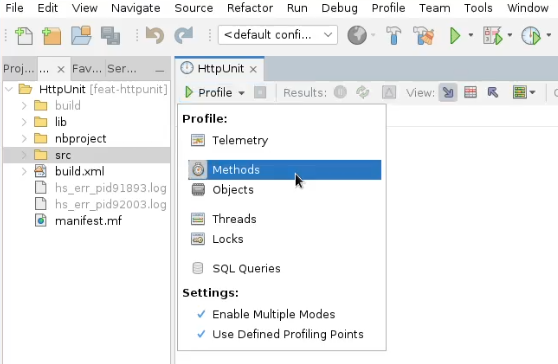
\includegraphics[width=0.7\textwidth]{screenshots/main-1.png}
    \caption{Выбор режима профилирования методов.}
  \end{figure}

  \item Ждём около пяти минут, чтобы накопилась статистика. После анализируем дерево вызовов в отображении Forward Calls и замечаем, что в потоке с методом Main \( 96.3\% \) реального времени занимает ожидание потока.
  
  Стоит отметить, что эта операция почти не занимает процессорное время: по тем же данным его доля составляет лишь \( 0.1\% \) от приложения, что подтверждает состояние ожидания, а не активных вычислений.

  \begin{figure}[H]
    \centering
    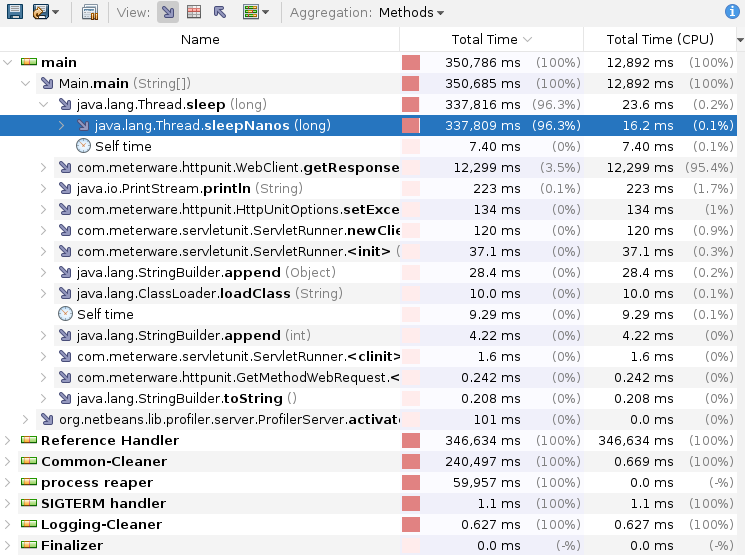
\includegraphics[width=0.7\textwidth]{screenshots/main-2.png}
    \caption{Анализ дерева вызовов методов.}
  \end{figure}

  \item Изучаем исходный код метода \texttt{main}, чтобы найти вызов метода \texttt{sleep} и~определить целесообразность его применения.

  \begin{lstlisting}[caption=Листинг метода \texttt{main} из класса \texttt{Main}.]
public static void main(String[] args) {
    try {
        HttpUnitOptions.setExceptionsThrownOnScriptError(false);
        ServletRunner sr = new ServletRunner();
        sr.registerServlet("myServlet", HelloWorld.class.getName());
        ServletUnitClient sc = sr.newClient();
        int number = 1;
        WebRequest request = new GetMethodWebRequest("http://test.meterware.com/myServlet");
        while (true) {
            WebResponse response = sc.getResponse(request);
            System.out.println("Count: " + number++ + response);
            java.lang.Thread.sleep(200); // it's here!
        }
    } catch (InterruptedException ex) {
        Logger.getLogger("global").log(Level.SEVERE, null, ex);
    } catch (MalformedURLException ex) {
        Logger.getLogger("global").log(Level.SEVERE, null, ex);
    } catch (IOException ex) {
        Logger.getLogger("global").log(Level.SEVERE, null, ex);
    } catch (SAXException ex) {
        Logger.getLogger("global").log(Level.SEVERE, null, ex);
    }
}
\end{lstlisting}
\end{enumerate}

\subsubsubsection{Пути устранения проблемы}

С одной стороны, искусственная задержка \texttt{Thread.sleep(200)} в бесконечном цикле не просто так: она предотвращает избыточную утилизацию процессора сетевыми запросами и делает логгирование читаемым для разработчика во время отладки.

С другой стороны, этот вызов искажает результаты профилирования, забирая на себя практически всё реальное время выполнения потока в дампах.

Экспериментальное удаление задержки показало, что встроенный профайлер NetBeans в текущем окружении не справляется с потоком генерируемых событий. Спустя 20 секунд работы агент профилирования аварийно завершается с кодом ошибки 134 (сигнал \texttt{SIGABRT})

\begin{figure}[H]
  \centering
  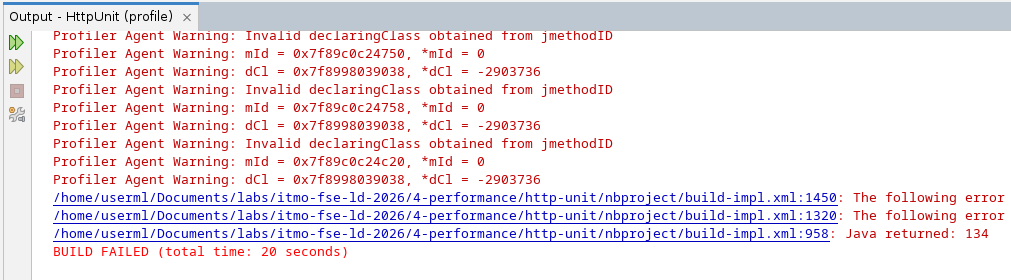
\includegraphics[width=0.7\textwidth]{screenshots/main-4.png}
  \caption{Ошибка агента профилирования при отключении задержки.}
\end{figure}

При этом тестирование стабильности приложения без профайлера в аналогичном окружении подтвердило его полную работоспособность: программа успешно и бездефектно обрабатывает десятки тысяч запросов в секунду.

\begin{figure}[H]
  \centering
  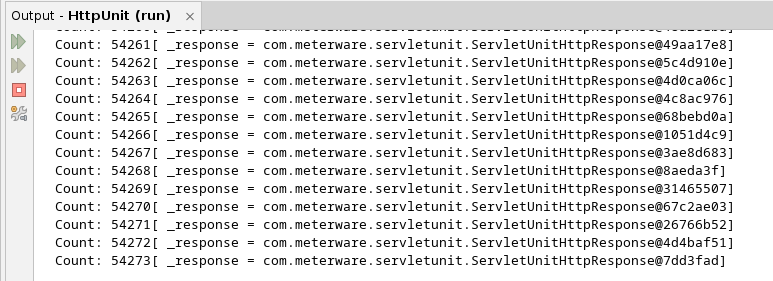
\includegraphics[width=0.7\textwidth]{screenshots/main-5.png}
  \caption{Нормальный ход обновлённой программы.}
\end{figure}

Так как обнаруженное узкое место является намеренным архитектурным ограничением для отладки, а нестабильность при его удалении вызвана исключительно ограничениями самого инструмента профилирования, принято решение оставить текущую реализацию без изменений при работе с данным профилировщиком.

\subsubsection{Избыточная активность сборщика мусора}

\subsubsubsection{Описание проблемы}

Наблюдается высокая частота вызова GC из-за накопления неиспользуемых элементов. Это снижает общую пропускную способность системы и впоследствии приводит к падению программы из-за переполнения памяти.

\subsubsubsection{Алгоритм локализации проблемы}

\begin{enumerate}
  \item Временное отключение задержки между итерациями в главном цикле приложения для ускорения воспроизведения потенциальной утечки памяти в другом инструменте, отличном от профилировщика NetBeans.
  \item Запускаем VisualVM и подключаемся к JVM-процессу исследуемой программы.
  \begin{figure}[H]
    \centering
    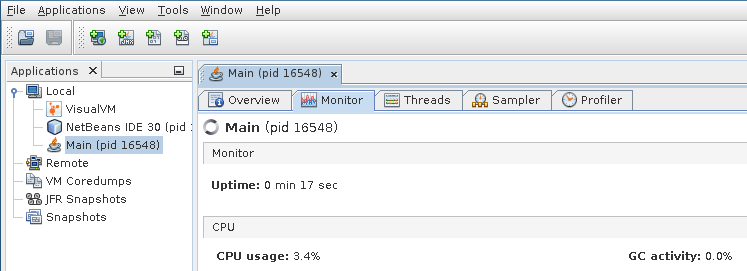
\includegraphics[width=0.7\textwidth]{screenshots/gc-1.png}
    \caption{Подключение к исследуемому процессу в VisualVM.}
  \end{figure}
  \item Мониторим состояние системы в течение времени и наблюдаем просадку производительности приложения вместе с высоким процентом времени CPU, которое тратится на сборку мусора.
  \begin{figure}[H]
    \centering
    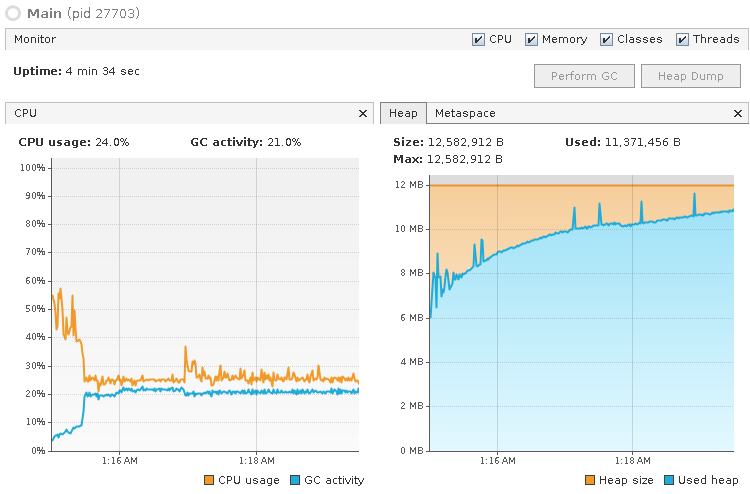
\includegraphics[width=0.7\textwidth]{screenshots/gc-fail.png}
    \caption{Фиксация высокой нагрузки на GC}
  \end{figure}
  \item Спустя некоторое время обнаруживаем падение программы из-за исчерпания доступного пространства в куче:
  \begin{figure}[H]
    \centering
    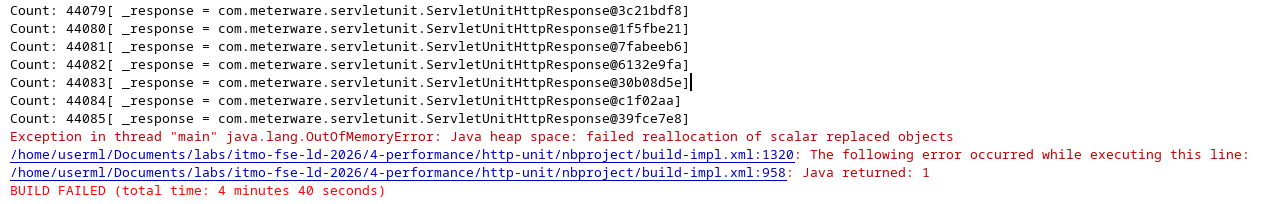
\includegraphics[width=0.7\textwidth]{screenshots/gc-with-1-lat.png}
    \caption{Аварийное завершение программы с ошибкой \texttt{OutOfMemoryError}.}
  \end{figure}
  \item Снимаем дамп памяти незадолго до критического сбоя и переключаем интерфейс профайлера в режим детального анализа объектов.
  \begin{figure}[H]
    \centering
    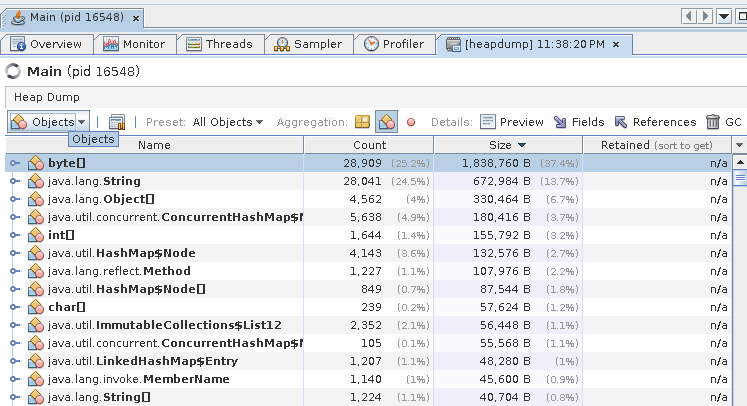
\includegraphics[width=0.7\textwidth]{screenshots/gc-3.png}
    \caption{Анализ полученного дампа кучи.}
  \end{figure}
  \item Включаем агрегацию по отдельным экземплярам классов: обнаруживаем статическую коллекцию \texttt{\_errorMessages} с большим количеством элементов, которая принадлежит используемой библиотеке.
  \begin{figure}[H]
    \centering
    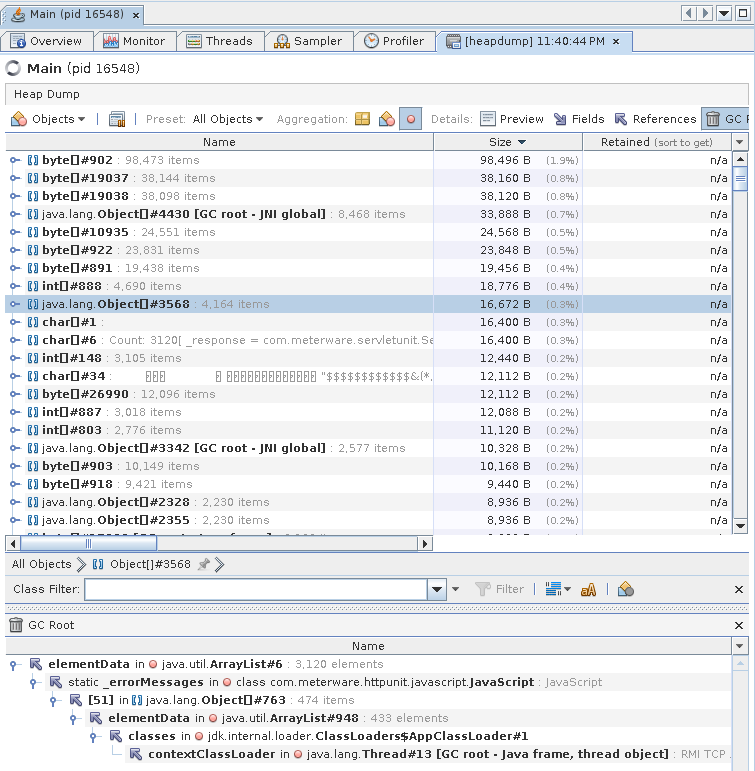
\includegraphics[width=0.7\textwidth]{screenshots/gc-4.png}
    \caption{Выявление объекта-виновника утечки памяти.}
  \end{figure}
  \item Изучаем исходный код и обнаруживаем, что класс \texttt{JavaScript} аккумулирует логи ошибок в статическом массиве, который не очищается автоматически. Освобождение памяти возможно только через явный вызов метода \texttt{HttpUnitOptions.clearScriptErrorMessages()}, который на данный момент отсутствует в основном цикле обработки.
\begin{lstlisting}[caption=Листинг класса JavaScript.]
public class JavaScript {
  // ...
  private static ArrayList _errorMessages = new ArrayList();
  // ...
  static void clearErrorMessages() {
    _errorMessages.clear();
  }
  // ...
}
\end{lstlisting}

\begin{lstlisting}[caption=Листинг класса JavaScriptEngineFactory.]
public class JavaScriptEngineFactory implements ScriptingEngineFactory {
  // ...
  public void clearErrorMessages() {
    JavaScript.clearErrorMessages();
  }
}
\end{lstlisting}

\begin{lstlisting}[caption=Листинг класса HttpUnitOptions.]
public abstract class HttpUnitOptions {
  /**
    * Determines whether script errors result in exceptions or warning messages.
    */
  public static void setExceptionsThrownOnScriptError( boolean throwExceptions ) {
    _exceptionsThrownOnScriptError = throwExceptions;
    getScriptingEngine().setThrowExceptionsOnError( throwExceptions );
  }
  /**
    * Returns the accumulated script error messages encountered. Error messages are accumulated only
    * if 'throwExceptionsOnError' is disabled.
    */
  public static String[] getScriptErrorMessages() {
    return getScriptingEngine().getErrorMessages();
  }
  /**
    * Clears the accumulated script error messages.
    */
  public static void clearScriptErrorMessages() {
      getScriptingEngine().clearErrorMessages();
  }

  private static boolean _exceptionsThrownOnScriptError = true;
}
\end{lstlisting}
\end{enumerate}

\subsubsubsection{Пути устранения проблемы}

Поскольку в основном цикле выполняется проверка корректности функционирования библиотеки, изменять общую стратегию обработки ошибок на генерацию исключений нецелесообразно.

В качестве оптимального решения было выбрано добавление вызова метода \texttt{HttpUnitOptions.clearScriptErrorMessages()} в конце каждой итерации цикла для принудительного освобождения буфера сообщений.

В результате повторный запуск и мониторинг показали стабильную и предсказуемую работу сборщика мусора без деградации памяти:

\begin{figure}[H]
  \centering
  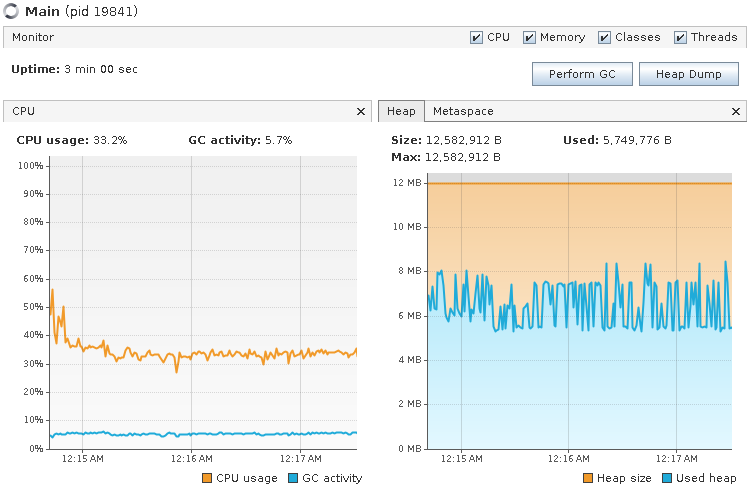
\includegraphics[width=0.7\textwidth]{screenshots/gc-5.png}
  \caption{Стабилизация работы GC после исправления.}
\end{figure}